
\begin{center}
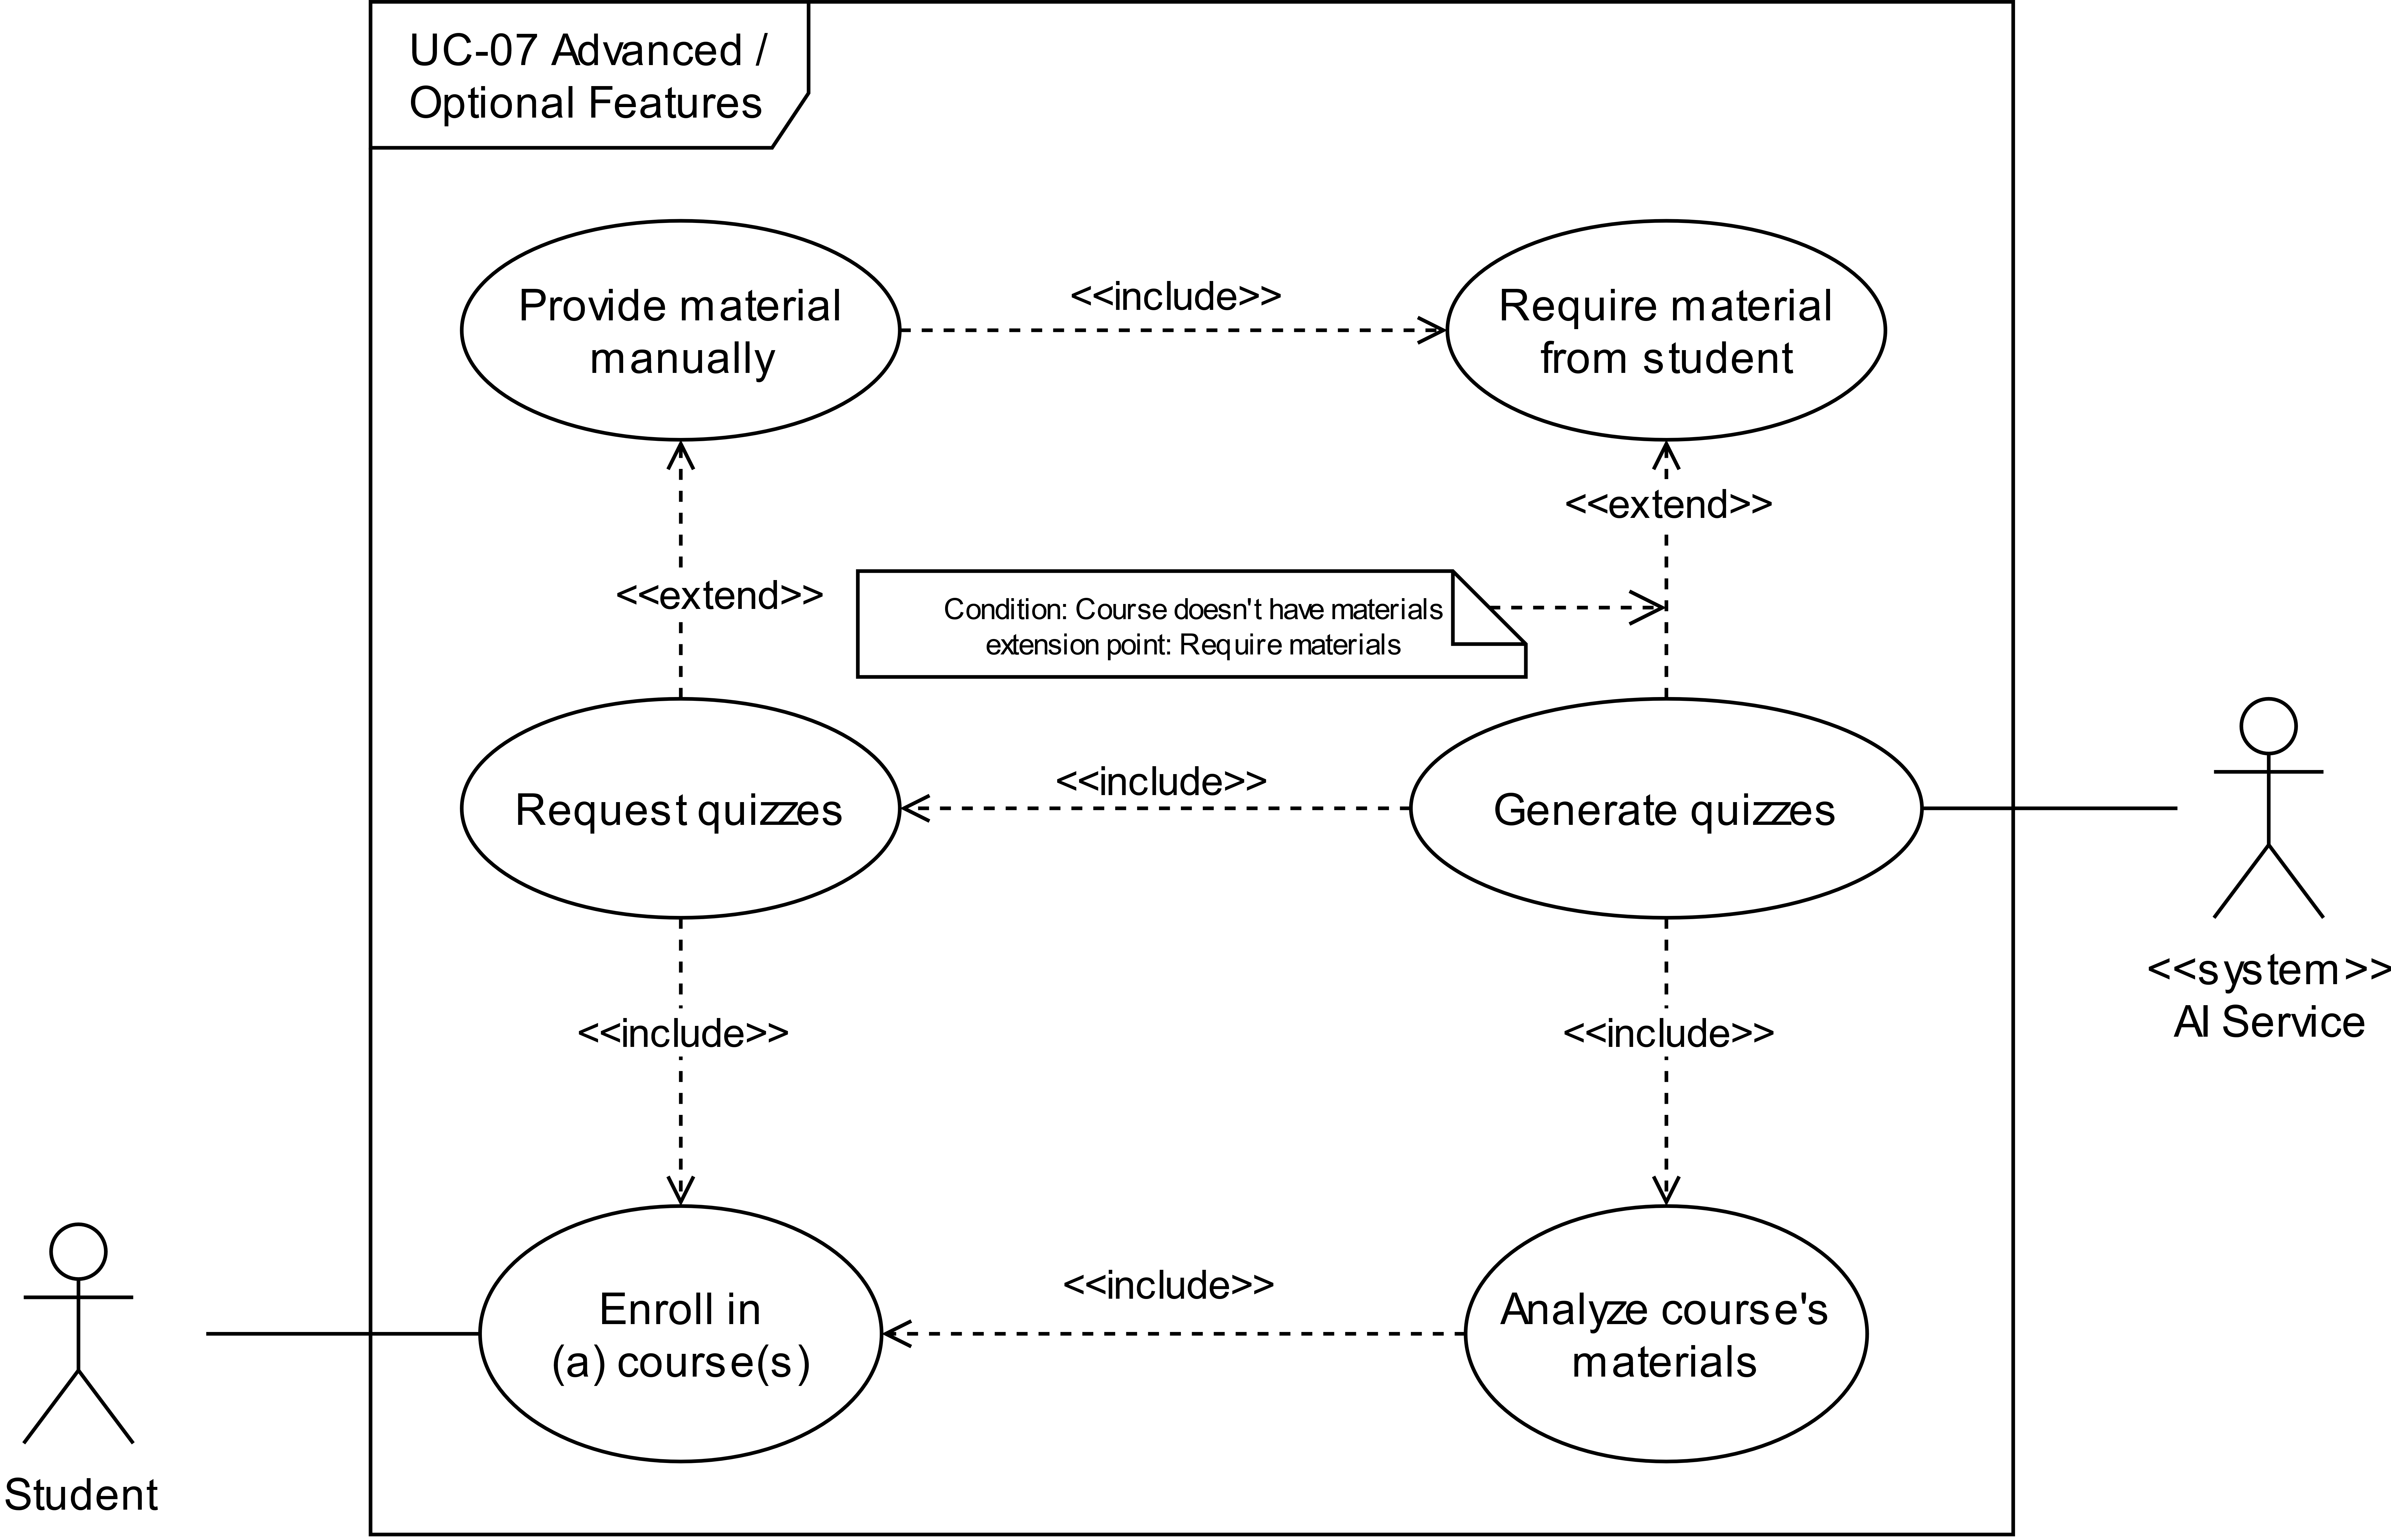
\includegraphics[width=0.9\linewidth]{images/UC-07.png}
\end{center}

\begin{center}
\textbf{Figure 8:}  AI-generated review quizzes
\end{center}

\begin{table}[h!]
\centering
\begin{tabular}{|p{3cm}|p{11cm}|}
\hline
\textbf{Use-case ID} & UC-07 \\
\hline
\textbf{Use-case name} & AI-generated review quizzes \\
\hline
\textbf{Use-case overview} & Provide students with quizzes related to the courses they are enrolling. \\
\hline
\textbf{Actors} & Students, AI service \\
\hline
\textbf{Preconditions} & 
1. The system is running. \newline
2. Internet connection is available. \newline
3. AI service must be available. \newline
4. The courses must have learning materials uploaded by tutors. \\
\hline
\textbf{Trigger} & Students use the AI-based quiz generation function. \\
\hline
\textbf{Steps} & 
1. Retrieve uploaded course materials of the course. \newline
2. Process and analyze the content with AI. \newline
3. Search the internet for related academic resources and quizzes. \newline
4. Generate quiz questions covering the key topics. \newline
5. Display the quiz to the requested students. \\
\hline
\textbf{Postconditions} & 
1. The quizzes are displayed on the screen of the requested students, and they can download the quizzes as a document file. \newline
2. The quizzes can be available until the end of the login session of the requested students, or until they finished the course if they chose to save the quizzes \\
\hline
\textbf{Alternative Flows} & 
- If the course doesn't have any learning materials, notify the user and request them for manual typing in key topics needed for review.
A1: Invalid login → Access denied with error message. \\
\hline
\textbf{Exception Flow} & 
1. If AI service isn't available, display an error. \\
\hline
\end{tabular}
\caption{Use Case UC-07: AI-generated review quizzes}
\end{table}
